\subsection{Preprocessing techniques}
In this section, we consider the attack information as noise in the image. We assume attackers tend to control the magnitude of their attacks so as not to be detected by the system, but make them effective enough to misguide the system to the wrong results. We then make use of this effect, and consider the problem from the image preprocessing perspective. We use different approaches, rescaling, bit-depth reduction and total variation, to remove the attack or adversarial perturbations in the input data before we fit into the net, and also try to maintain enough information for our net to give the right results.

\subsubsection{Bit-Depth Reduction} %reference needed here
Bit-Depth reduction approach is to reduce the color depth in bits. We know that each RGB channel has 8-bits, which is possible to be reduced. We then consider removing the noise by reducing the original 8-bit images to fewer bits, as a try to remove the adversarial attack but not significantly destroying the recognisability of the images. 

Before we introduce the way doing bit-depth reduction, we notice that our input values are in the range [0,1]. Then more specifically, for reducing from 8 bits to i bits, we first multiply the input data by ($2^i - 1$),then round to zeros, and scale the values back to the the range [0,1]. Hence we successfully reduce the information capacity from the original 8-bit to i-bit with the critical step of integer rounding. 

\begin{figure}[h!]
	\centering
	\begin{subfigure}{.35\textwidth}
		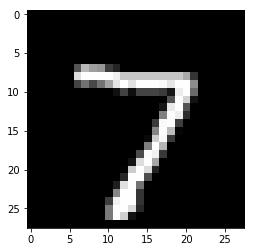
\includegraphics[width=\textwidth]{original7.png}
		\caption{the original image}
		\label{fig: bit-depth reduction 1}
	\end{subfigure}
	\begin{subfigure}{.35\textwidth}
		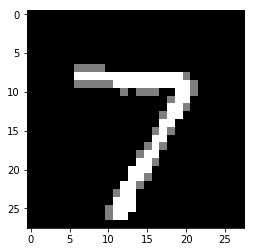
\includegraphics[width=\textwidth]{bit1-7.png}
		\caption{bit-one image}
		\label{fig: bit-depth reduction 8}
	\end{subfigure}
	\caption{Bit-depth reduction image}
\end{figure}

We can see for MNIST database, even we reduce the color depth to just 1 bit, it is very clear and does not introduce human-observable loss. But for images in colored ImageNet, it do shows significant loss when we reduce the bit-depth to be less than 4, which can also be inferred from the decrease in the accuracy in the following results section. 

\subsubsection{Total Variation}

